% introduction.tex

\section{INTRODUCTION}

\subsection{BACKGROUND OF THE PROJECT}

    To address these issues in sponsorship billing, which persists in the field, and the need to have reliable financial records, this study proposes an integration-first \textbf{SPONSOR MANAGEMENT AND LETTER OF GUARANTEE (LoG) COVERAGE INTEGRATION SYSTEM FOR INTERNATIONAL SCHOOL MANILA (ISM)}. The system does not look at sponsorship coverage as a local system, it also looks at it as a common institutional reference. It utilizes a centralized \textbf{Sponsor Master} and a uniform rules engine to cover the rules and parameters for student charges, as well as uniform identifiers that are synchronized across \textbf{PowerSchool} as the Student Information System (SIS) that holds the primary student profile, \textbf{NetSuite} as the finance system, which records charges and maintains the student ledger, the in-house \textbf{Student Charging Portal}, which processes charges by students, and the \textbf{Online Billing System}, which displays statements of account to parents and sponsors.
    
    International School Manila has four systems in place to bill students and these were implemented at various times due to various operational needs. \textbf{PowerSchool} contains enrollment and demographic information. The \textbf{Student Charging Portal} is used by front-line staff to make itemized charges. These charges are recorded in \textbf{NetSuite} and included in the student ledger for financial reporting. The ledger entries then become statements to parents and sponsors via the \textbf{Online Billing System}. Sponsorship billing is available in this multi-system environment and is backed by \textbf{Letters of Guarantee (LoG)} issued by sponsors to specify items and/or categories that they will sponsor.
    
    Each time a charge entry is added to the \textbf{Student Charging Portal}, operators review each LoG and decide if a line item is covered, and then indicate if it is a \textbf{Bill-To} by the sponsor or parent. These decisions go through the integration chain (charges are added into \textbf{NetSuite} and the \textbf{Online Billing System} shows the resulting statement of account for parents/sponsors). Staff use spreadsheet and 2 comma-separated value (CSV) files to manually match records between platforms and ensure the these platforms are synchronized.
 
    \begin{figure}[H]
        \centering
        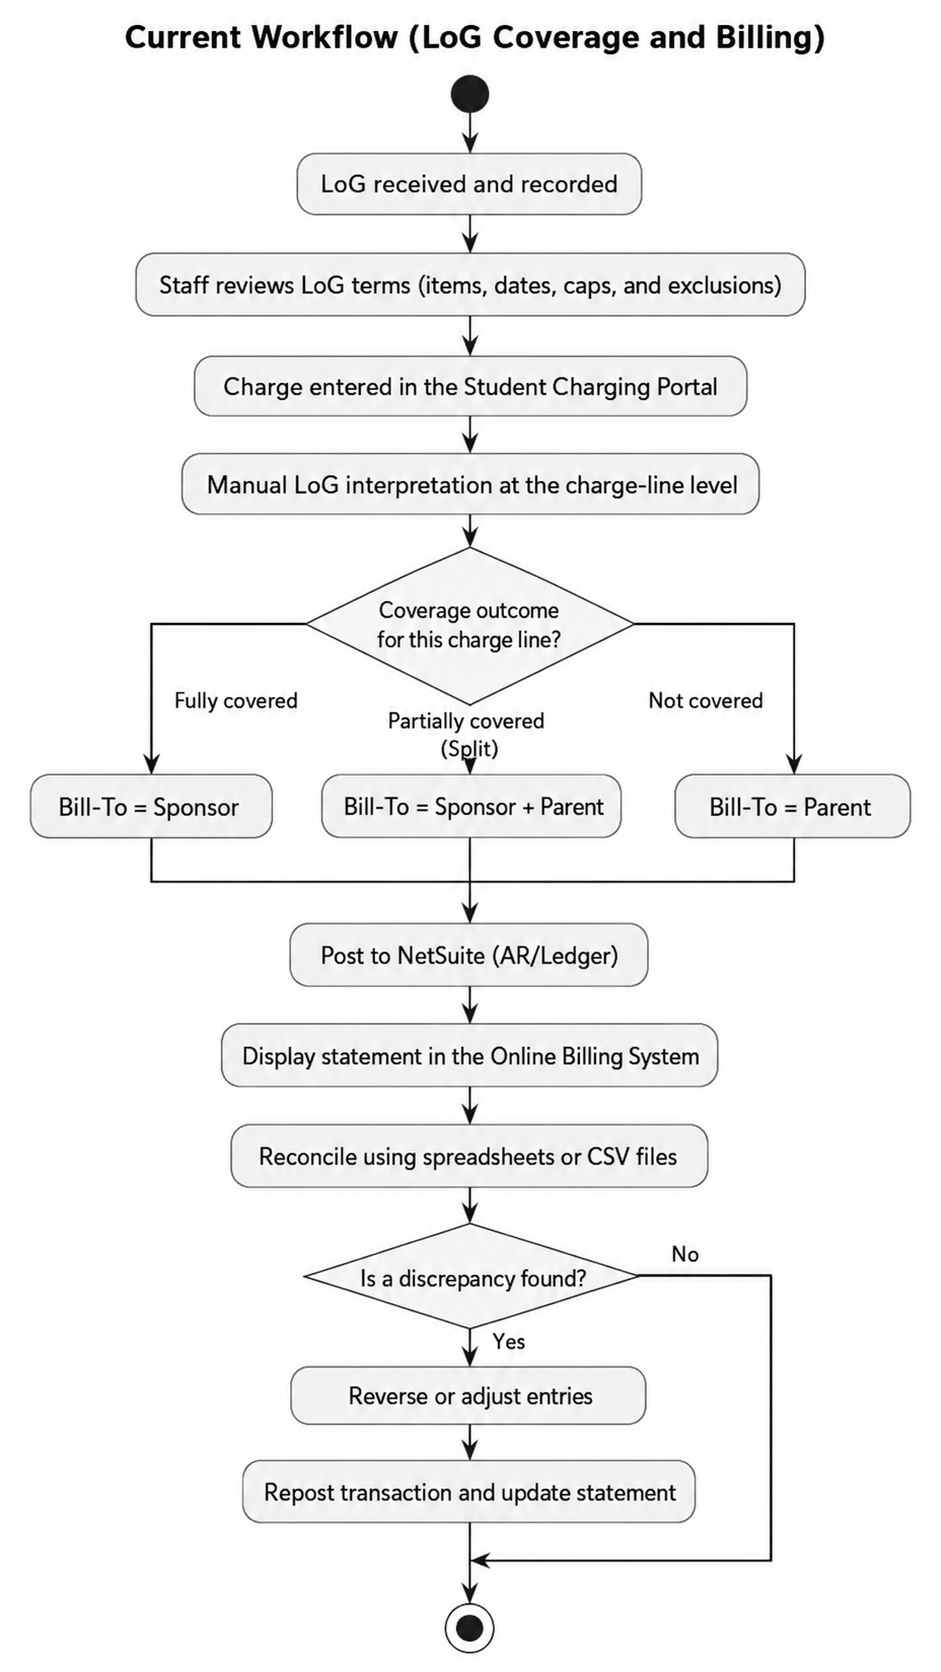
\includegraphics[width=0.95\linewidth,height=0.82\textheight,keepaspectratio]{images/Current Workflow.png}
        \caption{Current manual LoG coverage and billing workflow}
        \label{fig:current-workflow}
    \end{figure}

    \noindent Figure~\ref{fig:current-workflow} shows the current manual LoG coverage and billing workflow. The decision point clarifies the three possible outcomes for each charge line: full sponsor coverage, partial sponsor-parent coverage, and no sponsor coverage. These outcomes determine whether the Bill-To value is assigned to the sponsor, split between sponsor and parent, or assigned to the parent.

    With the passage of time, this manual interpretation and “file” based reconciliation has proven to be very problematic. This can make it hard to keep connections between spreadsheet references and unofficial notes with authoritative information. There is some variation among staff in how they interpret similar LoG provisions, and may result in a variety of \textbf{Bill-To} decisions on similar charges. Late postings, inaccurate postings, and missing documents decrease the trust in the student ledger, make reconciling more difficult and puts the institution at risk of audit and regulatory exposure. The concerns are set against a backdrop of a regulatory framework which demands accuracy, transparency and accountability.  

    Student information data needs to be synced from ISM to a third party SIS, billing capture to an in-house portal, statements to an in-house billing system and accounting data to a third-party finance system. It should also meet the requirement of the BIR policy on \textbf{‘Ease of Paying Taxes' (EoPT)} which requires the billing to be kept in a well documented and clear manner. A lack of person-centredness and disconnection around the amount of coverage of sponsorships within this context leads to tension in operations and governance. There are other solutions, but they have their own major cost/benefit considerations for ISM. 
    
    One way is to have a single vendor system which integrates student records, billing, ledgers and accounting in a single enterprise resource planning (ERP) application. This would drastically reduce the number of applications, but would require a massive migration, re-negotiation of current integrations and customization of ISM processes to meet the recommended processes of the vendor, which may differ from ISM's integration of \textbf{PowerSchool)}, \textbf{NetSuite)} and in-house processes. 
    
    The second option would be to use a dedicated sponsorship administration software or billing portals for sponsorships which are specifically created for billing and collections. These tools can aid in payment tracking but can continue to require manual interpretation of the charge when payments are inputted to the system and manual 4 reconciliation in a spreadsheet, thus perpetuating the lack of consistency charge-to-Bill. 
    
    The third approach is to continue improving the spreadsheet-based process with more stringent templates and more oversight of the review process. This approach remains ‘manual', labour intensive, scaleable and scalable to audit, however. These are not to be confused with the deployed \textbf{SPONSOR MANAGEMENT AND LETTER OF GUARANTEE (LoG) COVERAGE INTEGRATION SYSTEM FOR INTERNATIONAL SCHOOL MANILA (ISM))} which is not meant to take the place of the school's main systems. 
    
    It instead aims to address the issue of inconsistencies – lack of a single, rule-based sponsorship coverage source. The system does not replace \textbf{PowerSchool)}, \textbf{NetSuite)} or in-house portals, it is a shared institutional service to determine if there is coverage for the charge and if so, how to cover it is evaluated on every charge that is processed. This allows the line level, deterministic \textbf{Bill-To decisions} to be returned when the charges are entered, reflected as accurate transactions within \textbf{NetSuite)}, and displayed as a definite line of charge in the Online Billing System for parents and sponsors to see. By doing so, the deployed pilot system brings together the best of the existing landscape together with centralized logic and explainable decisions, offering a more practical, lower risk and institution-specific solution compared to undertaking a complete system replacement or a continued reliance on manual spreadsheets.
    \pagebreak

\subsection{DEFINITION OF TERMS}

\begin{description}
    \item[\textbf{AR}] Accounts Receivable.

    \item[\textbf{Azure}] Microsoft Azure, the cloud platform where system services and data are hosted.

    \item[\textbf{Bill-To Designation}] The ultimate decision of who the billing party is for a charge line item. This may be the sponsor, the parent, or both parties for downstream financial posting and statement presentation purposes.

    \item[\textbf{BIR EoPT}] Bureau of Internal Revenue Ease of Paying Taxes.

    \item[\textbf{Cashier}] Staff members who use the sponsor dropdown in PowerSchool (SIS) to tag a student's sponsor from the LoG system.

    \item[\textbf{Coverage Decision}] A determination outcome for a charge line item, classified as Covered, Split, or Not Covered, created when the charge item is created and stored with the reason code and rule version.

    \item[\textbf{Coverage Evaluation}] A rule-based process used to determine whether a sponsor covers a charge line item or charge line item category.

    \item[\textbf{Coverage Rule}] A deterministic rule specifying coverage by category or item, including limits, exceptions, and dates of coverage for the sponsor.

    \item[\textbf{CSV}] Comma-Separated Values, a flat-file format usually used to export and import data.

    \item[\textbf{Deterministic Rules Engine}] A rules-based evaluation component that makes consistent coverage decisions using the same inputs, explicit rule priorities, constraints, and computation logic, without using predictive modeling.

    \item[\textbf{ERP}] Enterprise Resource Planning.

    \item[\textbf{Identifier}] A unique value used to match and synchronize records between systems, such as sponsor IDs and student IDs.

    \item[\textbf{International School Manila}] The school where the Sponsor Management and LoG Coverage Integration System was developed and piloted. 
    
    \item[\textbf{IT Administrator Staff}] that installs integration and schedules. In the target state, they sync the records from the sponsors in the LoG system. 
    
    \item[\textbf{Ledger}] The financial history of charges and related transactions in the finance system. Letter of Guarantee (LoG) A letter from the sponsor outlining the amount of charges to be paid, coverage limits, dates, exclusions, supporting documentation etc.

    \item[\textbf{Letter of Guarantee (LoG)}] A document issued by the sponsor that details the extent of charges the sponsor will pay, including coverage limits, dates, exclusions, and supporting documentation.

    \item[\textbf{NetSuite}] The Finance and Accounting system used to record student charges and maintain the student ledger.

    \item[\textbf{NS}] NetSuite, also referred to as the Enterprise Resource Planning (ERP) system.

    \item[\textbf{OBS}] Online Billing System.

    \item[\textbf{Online Billing System}] The billing system that displays statements of account to parents and sponsors online.

    \item[\textbf{PowerSchool}] The Student Information System (SIS) that stores primary student enrollment and profile information.

    \item[\textbf{PS}] PowerSchool, the Student Information System.

    \item[\textbf{Reason Code}] A machine-readable label that explains a coverage or billing decision.

    \item[\textbf{Rules Engine}] The software component that applies coverage rules to charge entries and generates consistent and explainable results.

    \item[\textbf{SCP}] Student Charging Portal.

    \item[\textbf{SCP Operator}] Staff who enter student charges in SCP and use the coverage decision as the basis for deciding whether or not to cover the charge.

    \item[\textbf{Sponsor}] An outside organization, agency, or person who agrees to pay charges, in full or in part, for an assessed student under an approved Letter of Guarantee (LoG). Sponsorship is defined through billing-rule terms and conditions, including covered charge items or categories, coverage limits, effective dates, exclusions, required documentation, and allocation terms for sponsor and parent responsibility.

    \item[\textbf{Sponsor ID}] The unique identifier of a sponsor in this system.

    \item[\textbf{Sponsor-Parent Allocation}] The calculated way a charge amount is divided between sponsor responsibility and parent responsibility, in amounts and percentages, if applicable.

    \item[\textbf{Sponsor Master}] A single source of synchronized and consistent sponsors, attributes, identifiers and governance controls across PowerSchool, the Student Charging Portal, NetSuite and the Online Billing System.

    \item[\textbf{Statement of Account (SOA)}] An itemized billing statement that includes charges and parent-sponsor responsibilities.

    \item[\textbf{Student Charging Portal}] An in-house system used by staff to create and submit itemized student charges.

    \item[\textbf{Student Information System (SIS)}] Software used to store student enrollment, demographic, and profile information.

    \item[\textbf{Transaction}] A recorded financial event in the finance system, such as a charge entry, that is also shown in billing statements.
\end{description}
\pagebreak

\subsection{OBJECTIVES}

\subsubsection{General Objective}

    To create and implement an \textbf{INTEGRATED SPONSOR MANAGEMENT AND LETTER OF GUARANTEE (LoG) COVERAGE INTEGRATION SYSTEM FOR INTERNATIONAL SCHOOL MANILA (ISM)} that will automate the process of covering Student Charging Portal (SCP) Letter of Guarantee (LoG) in the PowerSchool system.

\subsubsection{Specific Objectives}

\begin{enumerate}
    \item To ensure \textbf{PowerSchool}, \textbf{NetSuite}, the \textbf{Student Charging Portal}, and the \textbf{Online Billing System} are all synchronized and validate sponsor coverage using a common identifier and processing business events like create, update and merge.

    \item To have a real-time, explainable coverage determination in the \textbf{Student Charging Portal (SCP)} that relies on a deterministic rules engine that utilizes sponsor coverage rules when charge is posted and reason codes are provided as human-readable values when a \textbf{Bill-To} determination is made.

    \item To develop a \textbf{Sponsor Master} with centralized sponsor records, coverage policies, limits, effective dates, status values and identifiers that will be used to identify students and track financial transactions in \textbf{PowerSchool} and \textbf{NetSuite}.

    \item To record proper \textbf{Bill-To} in \textbf{NetSuite} and the \textbf{Online Billing System}, support BIR audit and compliance requirements, and record proper sponsor/parent allocation in student ledger and general ledger.

    \item To ensure data quality and governance in the \textbf{Sponsor Master}, by validating required fields, attributes for classification and by maintaining authoritative cross-system identifiers, and by utilizing duplicate detection and merge workflows.
\end{enumerate}

\subsection{SCOPE}

    This project involves implementing the analysis, design, and pilot implementation of the \textbf{SPONSOR MANAGEMENT AND LETTER OF GUARANTEE (LoG) COVERAGE INTEGRATION SYSTEM FOR INTERNATIONAL SCHOOL MANILA (ISM)} hosted on \textbf{Microsoft Azure}. It involves designing and implementing the \textbf{Sponsor Master} repository to store all the information required to maintain sponsor records, coverage attributes, and cross-system identifiers, as well as the development of a rules model for item- and category-level coverage along with limits and defined exceptions.
    
    It also involves real time evaluation of coverage in the \textbf{Student Charging Portal}, propagation to \textbf{NetSuite} for posting and maintaining the student ledger, and syncing to the \textbf{Online Billing System} as parent/sponsor statements of account containing covered vs. uncovered items. Statements contain sponsor and parent responsibility, governing rule and relevant metadata. The primary users of this are Cashiers and Student Charging Portal operators, NetSuite Finance and Accounting users, and authorized department and school level administrators (parent/sponsors viewing statements through Online Billing System).
    
    The project includes work on critical integration flows, coverage evaluation logic, necessary user interface elements to test coverage preview and explanations in the \textbf{Student Charging Portal}, and control and logging of elements that aid review of sponsor-related transactions.

\subsection{LIMITATIONS}

    The pilot phase of the \textbf{SPONSOR MANAGEMENT AND LETTER OF GUARANTEE (LoG) COVERAGE INTEGRATION SYSTEM FOR INTERNATIONAL SCHOOL MANILA (ISM)} will not be hardened for full production until the next stage. The study deals with integration and coverage assessment, but is not predictive analytics, financial forecasting or optimizing sponsor portfolios. A comprehensive User Interface (UI) redesign of \textbf{PowerSchool}, \textbf{NetSuite} or the \textbf{Online Billing System} is not included; it is assumed that those systems will have their current interfaces with the exception of a few enhancements that will appear on the surface coverage information.
    
    Integration relies on the Application Programming Interfaces and secure file-based exchange that is provided by \textbf{PowerSchool}, \textbf{NetSuite} and in-house systems. Some of these interfaces might impose constraints that could affect real-time synchronization, and for some data sets, scheduled or batched updates could be necessary. Historical information on sponsorships and subsequent restatement of past sponsorships is not provided. The validation was based on representative, deidentified data along with structured user acceptance testing (UAT) that aligned with existing \textbf{Letters of Guarantee (LoG)}.
    
    Other topics such as performance tuning, advanced monitoring, DR and HA solutions were covered only as would be needed for a deployed pilot, and there is still work to be done before going to full production. The project has no plans to modify the rules for how payments are calculated, sponsor contracts, or basic business logic other than what is required to program in existing coverage agreements into the rules engine and \textbf{Sponsor Master}.
    